% Options for packages loaded elsewhere
\PassOptionsToPackage{unicode}{hyperref}
\PassOptionsToPackage{hyphens}{url}
%
\documentclass[
]{book}
\usepackage{amsmath,amssymb}
\usepackage{lmodern}
\usepackage{iftex}
\ifPDFTeX
  \usepackage[T1]{fontenc}
  \usepackage[utf8]{inputenc}
  \usepackage{textcomp} % provide euro and other symbols
\else % if luatex or xetex
  \usepackage{unicode-math}
  \defaultfontfeatures{Scale=MatchLowercase}
  \defaultfontfeatures[\rmfamily]{Ligatures=TeX,Scale=1}
\fi
% Use upquote if available, for straight quotes in verbatim environments
\IfFileExists{upquote.sty}{\usepackage{upquote}}{}
\IfFileExists{microtype.sty}{% use microtype if available
  \usepackage[]{microtype}
  \UseMicrotypeSet[protrusion]{basicmath} % disable protrusion for tt fonts
}{}
\makeatletter
\@ifundefined{KOMAClassName}{% if non-KOMA class
  \IfFileExists{parskip.sty}{%
    \usepackage{parskip}
  }{% else
    \setlength{\parindent}{0pt}
    \setlength{\parskip}{6pt plus 2pt minus 1pt}}
}{% if KOMA class
  \KOMAoptions{parskip=half}}
\makeatother
\usepackage{xcolor}
\IfFileExists{xurl.sty}{\usepackage{xurl}}{} % add URL line breaks if available
\IfFileExists{bookmark.sty}{\usepackage{bookmark}}{\usepackage{hyperref}}
\hypersetup{
  pdftitle={Tools for human-screen interactions},
  pdfauthor={cjlortie},
  hidelinks,
  pdfcreator={LaTeX via pandoc}}
\urlstyle{same} % disable monospaced font for URLs
\usepackage{longtable,booktabs,array}
\usepackage{calc} % for calculating minipage widths
% Correct order of tables after \paragraph or \subparagraph
\usepackage{etoolbox}
\makeatletter
\patchcmd\longtable{\par}{\if@noskipsec\mbox{}\fi\par}{}{}
\makeatother
% Allow footnotes in longtable head/foot
\IfFileExists{footnotehyper.sty}{\usepackage{footnotehyper}}{\usepackage{footnote}}
\makesavenoteenv{longtable}
\usepackage{graphicx}
\makeatletter
\def\maxwidth{\ifdim\Gin@nat@width>\linewidth\linewidth\else\Gin@nat@width\fi}
\def\maxheight{\ifdim\Gin@nat@height>\textheight\textheight\else\Gin@nat@height\fi}
\makeatother
% Scale images if necessary, so that they will not overflow the page
% margins by default, and it is still possible to overwrite the defaults
% using explicit options in \includegraphics[width, height, ...]{}
\setkeys{Gin}{width=\maxwidth,height=\maxheight,keepaspectratio}
% Set default figure placement to htbp
\makeatletter
\def\fps@figure{htbp}
\makeatother
\setlength{\emergencystretch}{3em} % prevent overfull lines
\providecommand{\tightlist}{%
  \setlength{\itemsep}{0pt}\setlength{\parskip}{0pt}}
\setcounter{secnumdepth}{5}
\usepackage{booktabs}
\ifLuaTeX
  \usepackage{selnolig}  % disable illegal ligatures
\fi
\usepackage[]{natbib}
\bibliographystyle{apalike}

\title{Tools for human-screen interactions}
\author{cjlortie}
\date{}

\begin{document}
\maketitle

{
\setcounter{tocdepth}{1}
\tableofcontents
}
\hypertarget{screen-adaptation-theory}{%
\chapter{Screen adaptation theory}\label{screen-adaptation-theory}}


\includegraphics[width=4in,height=\textheight]{./sat.png}

\hypertarget{context}{%
\subsection*{Context}\label{context}}
\addcontentsline{toc}{subsection}{Context}

Screens are a portal to information and to one another. \href{https://datareportal.com/global-digital-overview}{Nearly 5 billion people as of 2022 use the internet}. Treating screens and digital time only as a pathology neglects the inherent capacity for screens as a tool to promote higher levels of performance and novel approaches to problem solving. \href{https://www.frontiersin.org/articles/10.3389/fpsyg.2017.01335/full}{Mental models and the associated cognitive architecture} that we frame conceptually to decision making is critical for better choices. The screen adaptation theory (SAT) is proposed herein as a heuristic to enable individuals to use evidence and structured thinking in approaching screen time decisions.

Screens are a place. Going to work, visiting friends, visiting the library, and many other key personal tasks and professional functions are done via screens. It can seem trivial, but labeling these choices, explicitly, provides a sense of coherence and purpose. Screens as a place also provides context and ecology. Adaptation is the sum of traits that an individual possesses or develops that promote survival or higher levels of relative performance without those traits. The goal must be to amplify and identify traits that mitigate the real costs of screens and tip the net sum to positive and higher levels of performance. Theory is a set of principles. Many discipline support screens as a place and an adaptationist programme for screen time use. Source theory and scientific evidence depending the on specific context and choice.

\hypertarget{learning-outcomes}{%
\subsection*{Learning outcomes}\label{learning-outcomes}}
\addcontentsline{toc}{subsection}{Learning outcomes}

\begin{enumerate}
\def\labelenumi{\arabic{enumi}.}
\tightlist
\item
  Develop a new mental model for screen time.\\
\item
  Explore and track decisions associated with screen time.\\
\item
  Examine individual costs and benefits of screens.
\end{enumerate}

\hypertarget{schedule}{%
\subsection*{Schedule}\label{schedule}}
\addcontentsline{toc}{subsection}{Schedule}

Here is an outline of the challenges proposed to explore these principles in this course.

\begin{tabular}{rll}
\toprule
challenge & focus & tasks\\
\midrule
1 & Screen adaptation theory & read screen adaptation theory, explore a few theories that support change in screen use, and track screen time for a week\\
2 & Ten simple rules & test interventions, individually for your personal and professional interactions with screens for a week\\
3 & How to do nothing & explore liminal time and spaces to recharge and reframe how you work and interact, test out an ecological paradigm for yourself\\
\bottomrule
\end{tabular}

\hypertarget{citation}{%
\subsection*{Citation}\label{citation}}
\addcontentsline{toc}{subsection}{Citation}

Lortie, CJ (2021): Nature hacks for life. figshare. Book. \url{https://doi.org/10.6084/m9.figshare.16879312.v1}

\hypertarget{license}{%
\subsection*{License}\label{license}}
\addcontentsline{toc}{subsection}{License}

This work is licensed under a Creative Commons Attribution-NonCommercial-ShareAlike 4.0 International License.

\hypertarget{challenge-time}{%
\subsection*{Challenge time}\label{challenge-time}}
\addcontentsline{toc}{subsection}{Challenge time}

Use \href{https://scholar.google.com}{Google Scholar} and do a few search with screen time and \ldots. for whatever personal challenge is most urgent. Screen time and memory or fatigue or focus or vision etc. Use the filter tool on the left to return hits from 2018 onwards.

Review \href{https://figshare.com/articles/presentation/Screen_attention_theory/19686291}{slide deck for screen adaptation theory}.

Read screen adaptation theory at Ideas in Ecology and Evolution.

Track screen time use even cursorily. There are digital tools and functions included in the operating system of many devices. Or, go old school and have fun with it using a kitchen timer, stopwatch, or clock.

\hypertarget{reflection-questions}{%
\subsection*{Reflection questions}\label{reflection-questions}}
\addcontentsline{toc}{subsection}{Reflection questions}

\begin{enumerate}
\def\labelenumi{\arabic{enumi}.}
\tightlist
\item
  Did any of the work associated with screen time resonate with your challenge? If so, did the evidence nudge or shift your model and thinking?
\item
  Do you use mental models for other dimensions of your life such as training, sleep, or performance? Does your employer or team adopt models for performance?
\item
  Did tracking confirm your assumptions on frequency and duration of screen time?
\end{enumerate}

\hypertarget{rules}{%
\chapter{Ten simple rules}\label{rules}}

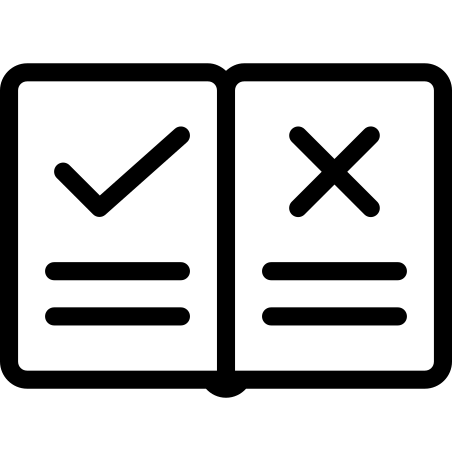
\includegraphics[width=3in,height=\textheight]{./rules.png}

\hypertarget{context-1}{%
\subsection*{Context}\label{context-1}}
\addcontentsline{toc}{subsection}{Context}

Rules help. Individually, simple rules can support \href{https://psycnet.apa.org/doiLanding?doi=10.1037\%2Fcap0000142}{emotional regulation} and belief. \href{https://journals.plos.org/ploscompbiol/article?id=10.1371/journal.pcbi.1006670}{Ten simple rules can be a magic number in science}, and this format of paper has been an incredibly successful medium for best practices and sharing expertise. Make, use, plan, and use data were the most common themes in the first 100 papers of work in using this heuristic model published in PLOS Computational Biology. \href{https://journals.plos.org/ploscompbiol/article?id=10.1371/journal.pcbi.1007706}{Ten simple rules for more objective decision-making} is a compelling and relevant examplar that supports structured decision making for screen time use. Break into smaller parts, mitigate bias, be transparent, and beware cognitive dissonance. These are salient principles for screen time decisions. Here, rules are proposed specific to screen time use using \href{https://journals.plos.org/ploscompbiol/article?id=10.1371/journal.pcbi.1003858}{principles for simple rules} including have ten, have a vision, and support with research as needed.

\textbf{Rules}

\begin{tabular}{rlll}
\toprule
rule & focus & description & evidence\\
\midrule
1 & Set intention & state purpose for every screen time instance; never ‘fill time’ with screens & {}[Screen time and young children: Promoting health and development in a digital world](https://academic.oup.com/pch/article/22/8/461/4392451)\\
2 & Track time & just a minute never happens; track time with some precision & {}[How Sedentary Are University Students? A Systematic Review and Meta-Analysis](https://link.springer.com/article/10.1007/s11121-020-01093-8)\\
3 & Manage attention & attention and perception are intimately linked; be mindful of how you spend attention whilst on a screen such as a video call, skip multi-tasking & {}[How to do nothing: resisting the attention economy](https://www.penguinrandomhouse.com/books/600671/how-to-do-nothing-by-jenny-odell/) and [Minds and brains of media multitaskers](https://www.pnas.org/doi/10.1073/pnas.1611612115)\\
4 & Block work & label and block work; cognitive task switching is costly & {}[Deep Work: Rules for Focused Success in a Distracted World](https://www.calnewport.com/books/deep-work/) and [The Impact of Digital Text](https://link.springer.com/chapter/10.1007/978-3-030-55152-0\_11)\\
5 & Plan breaks & every 20 minutes, take 20 seconds to look 20 feet away & {}[Digital eye strain: prevalence, measurement and amelioration](https://bmjophth.bmj.com/content/3/1/e000146)\\
\addlinespace
6 & Weigh costs and benefits & Transparently assess the potential costs and benefits of a specific task, function, or activity on a screen versus an alternative & {}[The Affect Heuristic in Judgments of Risks and Benefits](https://onlinelibrary.wiley.com/doi/10.1002/\%28SICI\%291099-0771\%28200001/03\%2913\%3A1\%3C1\%3A\%3AAID-BDM333\%3E3.0.CO\%3B2-S) and [Effects of Excessive Screen Time on Neurodevelopment, Learning, Memory, Mental Health, and Neurodegeneration: a Scoping Review](https://link.springer.com/article/10.1007/s11469-019-00182-2)\\
7 & Include collaboration & Synchronous online interactions are more effective in most instances & {}[Learning and Satisfaction in Webinar, Online, and Face-to-Face Instruction: A Meta-Analysis](https://www.frontiersin.org/articles/10.3389/feduc.2019.00092/full) and [The Role of Collaboration, Computer Use, Learning Environments, and Supporting Strategies in CSCL: A Meta-Analysis](https://journals.sagepub.com/doi/abs/10.3102/0034654318791584)\\
8 & Plan space & Real space matters; some spaces are conductive to deep work, others collaboration, others diffuse ideation & {}[Nomadic work and location independence: The role of space in shaping the work of digital nomads](https://onlinelibrary.wiley.com/doi/epdf/10.1002/hbe2.234)\\
9 & Experiment & Experiment with your screen time and green time with physical activity to boost performance & {}[Physical activity and screen time of children and adolescents before and during the COVID-19 lockdown in Germany: a natural experiment](https://www.nature.com/articles/s41598-020-78438-4) and [Can a ‘rewards-for-exercise app’ increase physical activity](https://bmcpublichealth.biomedcentral.com/articles/10.1186/s12889-021-10794-w)\\
10 & Set rules & Set rules for screen time use that work for you, your team, and your family; include rewards and positive alternatives; stack positive micro-habits & {}[A Goal-Theoretic Framework for Parental Screen-Time Monitoring Behavior](https://onlinelibrary.wiley.com/doi/abs/10.1111/jftr.12384) and [Ten simple rules for more objective decision-making](https://journals.plos.org/ploscompbiol/article?id=10.1371/journal.pcbi.1007706) and [Micro-habits for life-long learning](https://link.springer.com/article/10.1007/s00261-021-03185-7)\\
\bottomrule
\end{tabular}

\hypertarget{learning-outcomes-1}{%
\subsection*{Learning outcomes}\label{learning-outcomes-1}}
\addcontentsline{toc}{subsection}{Learning outcomes}

\begin{enumerate}
\def\labelenumi{\arabic{enumi}.}
\tightlist
\item
  Explore the behavioral trait reshaping capacity of life-hacking rules.\\
\item
  Examine some of the key evidence that supports your screen adaptation theory and personal development.\\
\item
  Change how you use screens.
\end{enumerate}

\hypertarget{challenge-time-1}{%
\subsection*{Challenge time}\label{challenge-time-1}}
\addcontentsline{toc}{subsection}{Challenge time}

\begin{enumerate}
\def\labelenumi{\arabic{enumi}.}
\tightlist
\item
  Review the ten simple rules. Experiment was one per day/week for a few days/weeks. Small changes first. Track its efficacy.\\
\item
  Develop and test a cognitive energy budget, daily. \href{https://figshare.com/articles/dataset/Cognitive_energy_budgets/19735525}{Here} is an example of a tracking exercise data dive for a scientist.
\item
  List any rules you were using for screen time (implicit or explicit).
\end{enumerate}

\hypertarget{reflection-questions-1}{%
\subsection*{Reflection questions}\label{reflection-questions-1}}
\addcontentsline{toc}{subsection}{Reflection questions}

\begin{enumerate}
\def\labelenumi{\arabic{enumi}.}
\tightlist
\item
  Document the extent that the rules improved your performance.\\
\item
  Do you have different screen time rules for your team or family than you currently adopt or would consider adopting?\\
\item
  Was there a place or time that screen time work was best supported for a specific work or professional task?
\end{enumerate}

\hypertarget{nothing}{%
\chapter{Do nothing}\label{nothing}}


\includegraphics[width=3in,height=\textheight]{./nothing.png}

\hypertarget{context-2}{%
\subsection*{Context}\label{context-2}}
\addcontentsline{toc}{subsection}{Context}

Doing nothing is an active process. It is not easy to `do' at all. The book \href{https://www.penguinrandomhouse.com/books/600671/how-to-do-nothing-by-jenny-odell/}{`How to do nothing: resisting the attention economy'} is a tranformative and novel text. Accepting and generating liminal spaces is one premise for the book. Another is that nature and place can support restoration and reframing of perception. Attention and perception are linked in this work, and it is proposed that deep listening or looking at things differently will enable a much more nuanced interaction with screens. We then think differently too. The premise of this book is not optimization. Nonetheless, using nature, art, and liminal experiences to be mindful of attention directly support better screen time decisions. A \href{https://www.frontiersin.org/articles/10.3389/fpsyg.2015.00500/full}{gate-and-key model for attention and perception} is developed throughout the text. We have an incredible perception network biologically in how we, see, hear, and feel. Attention drives what we perceive. This should be an active decision - always. Screens are one of the phenomenal metophorical nets that catch our attention in so many ways. Use attention to decide what to focus on. Resist in place. Continue to use screens and digital tools of course but do so much more wisely through attention management and liminal, preferably, natural/local/outdoor restoration time.

\hypertarget{learning-outcomes-2}{%
\subsection*{Learning outcomes}\label{learning-outcomes-2}}
\addcontentsline{toc}{subsection}{Learning outcomes}

\begin{enumerate}
\def\labelenumi{\arabic{enumi}.}
\tightlist
\item
  Understand the key trait-mediated interactions that you curate digitally and physically in your life.\\
\item
  Become aware of your daily digital routines.\\
\item
  Appreciate how attention drives perception with respect to screen time and beyond.
\end{enumerate}

\hypertarget{challenge-time-2}{%
\subsection*{Challenge time}\label{challenge-time-2}}
\addcontentsline{toc}{subsection}{Challenge time}

\begin{enumerate}
\def\labelenumi{\arabic{enumi}.}
\tightlist
\item
  Practice liminal and logical breaks. Walk to work. Try walking meetings or calls.
\item
  Try seeing things differently or hearing them via redirecting attention to novel components of a signal or information that an experience provides. This can include screens too - tool bars, ads, or any elements of digital work. Where do you focus and how do you listen? Apply this attention-focus awareness for meetings - real or virtual.\\
\item
  Read this \href{https://www.nytimes.com/2019/04/30/books/review/jenny-odell-how-to-do-nothing.html}{review of how to do nothing}.\\
\item
  Explore some the literature associated with \href{https://en.wikipedia.org/wiki/Nature_deficit_disorder}{nature deficit disorder}.\\
\item
  Review this \href{https://figshare.com/articles/presentation/How_to_do_nothing/19736179}{slide deck} on how to do nothing - actively.
\end{enumerate}

\hypertarget{reflection-questions-2}{%
\subsection*{Reflection questions}\label{reflection-questions-2}}
\addcontentsline{toc}{subsection}{Reflection questions}

\begin{enumerate}
\def\labelenumi{\arabic{enumi}.}
\tightlist
\item
  You are never alone in nature. Did this proposition resonante in any of the times you secured for a break/walk or mini-adventure between screen work instances. Did any of your affective components shift internally?\\
\item
  In your daily routine, was there `space' for attention to other experiences? Did you notice any opportunities that were already present for practiced awareness of the gate-and-key model but were unexploited?\\
\item
  Can you invoke some ecology (organismal-others-environment) thinking to improve your performance either through liminal moments or direct opportunities within the digital work that you do?
\end{enumerate}

  \bibliography{book.bib,packages.bib}

\end{document}
